\section{Characterisation of the signal and control regions}
\label{sec:yields}

A selection of relevant data/MC comparison plots for the signal and
control regions are presented here.  The event selection criteria
defining these regions are detailed in
Sec.~\ref{sec:selection}. Corrections applied to the simulated events
are discussed in Section~\ref{sec:mc-corrections}. The
distributions are shown separately according three \njet categories:
symmetric, asymmetric, and monojet. The distributions are intended to
provide a qualitative understanding of the simulation modelling for
key variables. However, the analysis is not sensitive due to the
reliance on simulation via ratios only (\ie transfer factors) and the
one-to-one mapping of (\njet,~\nb,~\scalht) binning between the
control and signal regions. For monojet, the distributions of
azimuthal angle of jets are included along with other key variables to
demonstrate the absence of beam halo effects. The simulated
distributions are normalized to an integrated luminosity of
36.4~$\ifb$ (the data/MC scale factors are also shown in all plots).

%In addition to distributions, the binned yields in the \mj, \mmj, and
%\gj control samples can be found in
%Tables~\ref{tab:yieldssep_mu_data_sym}-\ref{tab:yieldssep_mu_data_mono},
%\ref{tab:yieldssep_mumu_data_sym}-\ref{tab:yieldssep_mumu_data_mono},
%and \ref{tab:yieldssep_gj_data_sym}-\ref{tab:yieldssep_gj_data_mono},
%respectively, which correspond to an integrated luminosity of 12.9
%\ifb. 
%Breakdown of SM processes for some (\njet,~\nb,~\scalht) bins are shown in Tables
%~\ref{tab:yieldSM-signal} to ~\ref{tab:yieldSM-singlephoton}.
%Finally, Tables~\ref{tab:yieldsnodata_sig_comb_sym},
%\ref{tab:yieldsnodata_sig_comb_asym} and \ref{tab:yieldsnodata_sig_comb_mono} summarise the expected yields, as
%determined from simulation, in the signal region for an integrated
%luminosity of 12.9 \ifb.

%\clearpage
%\subsection{Breakdown of yields from various SM processes}
%\begin{longtable}{| c | c | c | c | c | c | c | c | c  | }
\caption{Summary of yields of each SM process} \label{tab:table} \\    \hline 
$n_{j}$~$n_{b}$~$H_{T}$ & $t\bar{t}$ & $W+jets$ & $Z \rightarrow \nu\nu$ & $DY+jets$ & $Single Top$ & $DiBoson$ & $Multijet$ & Total Yield\\ \hline 
eq2j eq0b 200 & 103.49 & 1026.57 & 1148.86 & 18.24 & 15.98 & 72.15 & 0.00 & 2385.28\\ \hline 
eq2j eq0b 250 & 74.63 & 1050.96 & 1312.16 & 16.09 & 15.33 & 74.25 & 10.11 & 2553.53\\ \hline 
eq2j eq0b 300 & 32.27 & 664.60 & 941.01 & 9.13 & 6.52 & 42.69 & 2.85 & 1699.07\\ \hline 
eq2j eq0b 350 & 12.65 & 395.06 & 569.00 & 5.50 & 1.62 & 17.06 & 1.33 & 1002.24\\ \hline 
eq2j eq0b 400 & 7.22 & 316.98 & 551.29 & 3.96 & 2.22 & 14.28 & 1.51 & 897.46\\ \hline 
eq2j eq0b 500 & 1.33 & 102.97 & 190.11 & 0.79 & 0.01 & 2.12 & 0.00 & 297.31\\ \hline 
eq2j eq0b 600 & 0.47 & 50.93 & 111.12 & 0.29 & 0.54 & 2.69 & 0.00 & 166.04\\ \hline 
eq2j eq0b 800 & 0.52 & 86.65 & 146.22 & 0.39 & 0.00 & 3.16 & 0.00 & 236.94\\ \hline 
eq3j eq1b 200 & 0.57 & 0.00 & 0.32 & 0.00 & 0.00 & 0.00 & 0.00 & 0.89\\ \hline 
eq3j eq1b 250 & 64.13 & 17.16 & 27.10 & 0.54 & 5.36 & 1.22 & 0.00 & 115.51\\ \hline 
eq3j eq1b 300 & 122.13 & 56.55 & 74.29 & 1.00 & 13.99 & 2.69 & 0.00 & 270.64\\ \hline 
eq3j eq1b 350 & 94.34 & 52.60 & 82.06 & 0.85 & 13.66 & 5.30 & 6.22 & 255.03\\ \hline 
eq3j eq1b 400 & 71.61 & 66.57 & 99.75 & 0.82 & 15.02 & 3.06 & 0.43 & 257.26\\ \hline 
eq3j eq1b 500 & 11.23 & 18.94 & 42.91 & 0.24 & 1.88 & 1.61 & 0.00 & 76.82\\ \hline 
eq3j eq1b 600 & 2.92 & 10.44 & 26.73 & 0.12 & 0.66 & 1.20 & 0.00 & 42.06\\ \hline 
eq3j eq1b 800 & 1.93 & 11.73 & 29.27 & 0.07 & 0.54 & 1.37 & 0.00 & 44.92\\ \hline 
eq4j eq2b 200 & 0.00 & 0.00 & 0.00 & 0.00 & 0.00 & 0.00 & 0.00 & 0.00\\ \hline 
eq4j eq2b 250 & 0.20 & 0.00 & 0.02 & 0.00 & 0.00 & 0.00 & 0.00 & 0.22\\ \hline 
eq4j eq2b 300 & 18.30 & 0.75 & 1.98 & 0.01 & 1.38 & 0.00 & 0.00 & 22.42\\ \hline 
eq4j eq2b 350 & 56.98 & 4.03 & 6.78 & 0.08 & 3.56 & 0.00 & 0.00 & 71.43\\ \hline 
eq4j eq2b 400 & 86.02 & 6.97 & 12.42 & 0.11 & 4.54 & 0.60 & 0.00 & 110.66\\ \hline 
eq4j eq2b 500 & 21.45 & 2.68 & 7.27 & 0.05 & 2.76 & 0.25 & 0.00 & 34.46\\ \hline 
eq4j eq2b 600 & 5.24 & 2.02 & 4.38 & 0.02 & 1.26 & 0.05 & 0.00 & 12.98\\ \hline 
eq4j eq2b 800 & 2.66 & 0.00 & 3.79 & 0.02 & 0.58 & 0.00 & 0.00 & 7.06\\ \hline 
ge5j eq0b 200 & 0.00 & 0.00 & 0.00 & 0.00 & 0.00 & 0.00 & 0.00 & 0.00\\ \hline 
ge5j eq0b 250 & 0.00 & 0.00 & 0.00 & 0.00 & 0.00 & 0.00 & 0.00 & 0.00\\ \hline 
ge5j eq0b 300 & 0.03 & 0.00 & 0.05 & 0.00 & 0.00 & 0.00 & 0.00 & 0.07\\ \hline 
ge5j eq0b 350 & 6.96 & 8.88 & 7.98 & 0.26 & 0.00 & 0.39 & 0.02 & 24.49\\ \hline 
ge5j eq0b 400 & 57.77 & 102.86 & 111.49 & 1.65 & 3.35 & 4.48 & 0.00 & 281.60\\ \hline 
ge5j eq0b 500 & 41.04 & 96.56 & 124.97 & 1.30 & 1.62 & 1.67 & 8.83 & 275.99\\ \hline 
ge5j eq0b 600 & 26.59 & 91.74 & 128.08 & 0.96 & 2.62 & 3.95 & 1.72 & 255.67\\ \hline 
ge5j eq0b 800 & 16.75 & 67.00 & 130.94 & 0.76 & 1.84 & 2.45 & 6.82 & 226.57\\ \hline 
    \hline 
    \hline 
\end{longtable}

%\clearpage
%
\begin{longtable}{| c | c | c | c | c | c | c  | }
\caption{Summary of yields of each SM process with green band correction for single mu control region} \label{tab:yieldSM-singlemu} \\    \hline 
$n_{j}$~$n_{b}$~$H_{T}$ & $t\bar{t}$ & $W+jets$ & $DY+jets$ & $Single Top$ & $DiBoson$ & $Multijet$\\ \hline 
eq2j eq0b 200 & 49.72 & 462.03 & 12.22 & 13.20 & 11.00 & 0.00\\ \hline 
eq2j eq0b 250 & 43.63 & 696.98 & 17.99 & 14.91 & 21.91 & 29.43\\ \hline 
eq2j eq0b 300 & 25.93 & 694.87 & 18.48 & 10.09 & 9.60 & 0.00\\ \hline 
eq2j eq0b 350 & 16.12 & 651.65 & 15.93 & 8.28 & 8.68 & 2.06\\ \hline 
eq2j eq0b 400 & 14.27 & 817.43 & 20.20 & 9.19 & 6.81 & 1.48\\ \hline 
eq2j eq0b 500 & 4.54 & 421.47 & 9.11 & 7.35 & 3.41 & 1.78\\ \hline 
eq2j eq0b 600 & 4.53 & 337.94 & 6.84 & 4.88 & 3.14 & 0.04\\ \hline 
eq2j eq0b 800 & 1.75 & 189.75 & 3.45 & 1.01 & 3.54 & 0.87\\ \hline 
eq3j eq1b 200 & 0.75 & 0.36 & 0.00 & 0.19 & 0.00 & 0.00\\ \hline 
eq3j eq1b 250 & 75.46 & 19.58 & 0.43 & 11.84 & 0.32 & 0.00\\ \hline 
eq3j eq1b 300 & 148.89 & 50.89 & 1.86 & 20.80 & 1.66 & 0.00\\ \hline 
eq3j eq1b 350 & 136.62 & 58.21 & 1.97 & 25.78 & 0.72 & 0.00\\ \hline 
eq3j eq1b 400 & 157.15 & 99.79 & 2.90 & 38.57 & 2.24 & 1.40\\ \hline 
eq3j eq1b 500 & 61.56 & 64.65 & 1.97 & 19.55 & 2.95 & 0.17\\ \hline 
eq3j eq1b 600 & 39.88 & 62.71 & 1.62 & 18.90 & 1.38 & 0.18\\ \hline 
eq3j eq1b 800 & 14.32 & 42.72 & 0.96 & 11.82 & 0.51 & 0.45\\ \hline 
eq4j eq2b 200 & 0.00 & 0.00 & 0.00 & 0.00 & 0.00 & 0.00\\ \hline 
eq4j eq2b 250 & 0.58 & 0.00 & 0.00 & 0.04 & 0.00 & 0.00\\ \hline 
eq4j eq2b 300 & 24.25 & 0.40 & 0.05 & 2.44 & 0.00 & 0.00\\ \hline 
eq4j eq2b 350 & 78.01 & 2.84 & 0.06 & 6.14 & 0.00 & 0.00\\ \hline 
eq4j eq2b 400 & 174.10 & 7.82 & 0.28 & 16.06 & 0.22 & 0.69\\ \hline 
eq4j eq2b 500 & 93.31 & 7.37 & 0.27 & 14.76 & 0.33 & 0.00\\ \hline 
eq4j eq2b 600 & 65.49 & 7.41 & 0.29 & 12.46 & 0.05 & 0.00\\ \hline 
eq4j eq2b 800 & 21.14 & 5.52 & 0.16 & 6.98 & 0.00 & 0.00\\ \hline 
ge5j eq0b 200 & 0.00 & 0.00 & 0.00 & 0.00 & 0.00 & 0.00\\ \hline 
ge5j eq0b 250 & 0.00 & 0.00 & 0.00 & 0.00 & 0.00 & 0.00\\ \hline 
ge5j eq0b 300 & 0.07 & 0.19 & 0.01 & 0.00 & 0.33 & 0.00\\ \hline 
ge5j eq0b 350 & 5.10 & 7.62 & 0.30 & 0.21 & 0.10 & 0.00\\ \hline 
ge5j eq0b 400 & 49.27 & 64.97 & 2.42 & 3.05 & 2.14 & 0.64\\ \hline 
ge5j eq0b 500 & 60.81 & 110.72 & 3.07 & 3.99 & 1.55 & 0.18\\ \hline 
ge5j eq0b 600 & 74.42 & 176.44 & 5.00 & 7.23 & 2.47 & 2.68\\ \hline 
ge5j eq0b 800 & 50.81 & 193.80 & 5.31 & 6.95 & 1.96 & 1.28\\ \hline 
    \hline 
    \hline 
\end{longtable}


%\clearpage
%
\begin{longtable}{| c | c | c | c | c | c | c  | }
\caption{Summary of yields of each SM process with green band correction for double mu control region} \label{tab:yieldSM-doublemu} \\    \hline 
$n_{j}$~$n_{b}$~$H_{T}$ & $t\bar{t}$ & $W+jets$ & $DY+jets$ & $Single Top$ & $DiBoson$ & $Multijet$\\ \hline 
eq2j eq0b 200 & 0.30 & 0.00 & 48.76 & 0.00 & 0.72 & 0.00\\ \hline 
eq2j eq0b 250 & 0.76 & 0.00 & 76.51 & 0.21 & 1.43 & 0.00\\ \hline 
eq2j eq0b 300 & 0.24 & 0.00 & 75.50 & 0.04 & 0.94 & 0.00\\ \hline 
eq2j eq0b 350 & 0.37 & 0.00 & 66.59 & 0.17 & 0.70 & 0.00\\ \hline 
eq2j eq0b 400 & 0.19 & 0.00 & 86.99 & 0.21 & 0.69 & 0.00\\ \hline 
eq2j eq0b 500 & 0.15 & 0.00 & 45.77 & 0.00 & 0.36 & 0.00\\ \hline 
eq2j eq0b 600 & 0.04 & 0.00 & 36.53 & 0.00 & 0.18 & 0.00\\ \hline 
eq2j eq0b 800 & 0.02 & 0.00 & 20.22 & 0.00 & 0.20 & 0.00\\ \hline 
eq3j eq1b 200 & 0.00 & 0.00 & 0.00 & 0.00 & 0.00 & 0.00\\ \hline 
eq3j eq1b 250 & 0.91 & 0.00 & 2.58 & 0.00 & 0.00 & 0.00\\ \hline 
eq3j eq1b 300 & 1.34 & 0.00 & 5.41 & 0.11 & 0.00 & 0.00\\ \hline 
eq3j eq1b 350 & 1.15 & 0.00 & 6.85 & 0.61 & 0.24 & 0.00\\ \hline 
eq3j eq1b 400 & 1.75 & 0.00 & 11.28 & 0.10 & 0.18 & 0.00\\ \hline 
eq3j eq1b 500 & 0.83 & 0.00 & 7.53 & 0.16 & 0.31 & 0.00\\ \hline 
eq3j eq1b 600 & 0.99 & 0.00 & 7.21 & 0.11 & 0.23 & 0.00\\ \hline 
eq3j eq1b 800 & 0.61 & 0.00 & 4.83 & 0.00 & 0.30 & 0.00\\ \hline 
eq4j eq2b 200 & 0.00 & 0.00 & 0.00 & 0.00 & 0.00 & 0.00\\ \hline 
eq4j eq2b 250 & 0.00 & 0.00 & 0.00 & 0.00 & 0.00 & 0.00\\ \hline 
eq4j eq2b 300 & 0.13 & 0.00 & 0.21 & 0.00 & 0.00 & 0.00\\ \hline 
eq4j eq2b 350 & 0.75 & 0.00 & 0.42 & 0.00 & 0.07 & 0.00\\ \hline 
eq4j eq2b 400 & 1.24 & 0.00 & 1.24 & 0.02 & 0.00 & 0.00\\ \hline 
eq4j eq2b 500 & 0.80 & 0.00 & 1.02 & 0.14 & 0.00 & 0.00\\ \hline 
eq4j eq2b 600 & 0.58 & 0.00 & 1.05 & 0.14 & 0.00 & 0.00\\ \hline 
eq4j eq2b 800 & 0.60 & 0.00 & 0.74 & 0.12 & 0.00 & 0.00\\ \hline 
ge5j eq0b 200 & 0.00 & 0.00 & 0.00 & 0.00 & 0.00 & 0.00\\ \hline 
ge5j eq0b 250 & 0.00 & 0.00 & 0.00 & 0.00 & 0.00 & 0.00\\ \hline 
ge5j eq0b 300 & 0.00 & 0.00 & 0.00 & 0.00 & 0.00 & 0.00\\ \hline 
ge5j eq0b 350 & 0.00 & 0.00 & 0.58 & 0.00 & 0.00 & 0.00\\ \hline 
ge5j eq0b 400 & 0.20 & 0.00 & 6.73 & 0.08 & 0.00 & 0.00\\ \hline 
ge5j eq0b 500 & 0.14 & 0.00 & 10.68 & 0.00 & 0.24 & 0.00\\ \hline 
ge5j eq0b 600 & 0.75 & 0.00 & 16.98 & 0.00 & 0.28 & 0.00\\ \hline 
ge5j eq0b 800 & 0.42 & 0.00 & 19.90 & 0.00 & 0.27 & 0.00\\ \hline 
    \hline 
    \hline 
\end{longtable}


%\clearpage
%\begin{longtable}{| c | c | c | c  | }
\caption{Summary of yields of each SM process} \label{tab:table} \\    \hline 
$n_{j}$~$n_{b}$~$H_{T}$ & $\gamma+jets$ & $Multijet$ & Total Yield\\ \hline 
eq2j eq0b 200 & 0.00 & 0.00 & 0.00\\ \hline 
eq2j eq0b 250 & 0.00 & 0.00 & 0.00\\ \hline 
eq2j eq0b 300 & 0.00 & 0.00 & 0.00\\ \hline 
eq2j eq0b 350 & 0.00 & 0.00 & 0.00\\ \hline 
eq2j eq0b 400 & 1529.97 & 38.85 & 1568.83\\ \hline 
eq2j eq0b 500 & 596.05 & 7.10 & 603.15\\ \hline 
eq2j eq0b 600 & 344.93 & 6.22 & 351.15\\ \hline 
eq2j eq0b 800 & 940.80 & 10.68 & 951.49\\ \hline 
eq3j eq1b 200 & 0.00 & 0.00 & 0.00\\ \hline 
eq3j eq1b 250 & 0.00 & 0.00 & 0.00\\ \hline 
eq3j eq1b 300 & 0.00 & 0.00 & 0.00\\ \hline 
eq3j eq1b 350 & 0.00 & 0.00 & 0.00\\ \hline 
eq3j eq1b 400 & 257.52 & 2.47 & 259.99\\ \hline 
eq3j eq1b 500 & 137.80 & 4.45 & 142.25\\ \hline 
eq3j eq1b 600 & 100.01 & 3.44 & 103.45\\ \hline 
eq3j eq1b 800 & 196.18 & 10.66 & 206.84\\ \hline 
eq4j eq2b 200 & 0.00 & 0.00 & 0.00\\ \hline 
eq4j eq2b 250 & 0.00 & 0.00 & 0.00\\ \hline 
eq4j eq2b 300 & 0.00 & 0.00 & 0.00\\ \hline 
eq4j eq2b 350 & 0.00 & 0.00 & 0.00\\ \hline 
eq4j eq2b 400 & 22.55 & 0.00 & 22.55\\ \hline 
eq4j eq2b 500 & 20.27 & 0.00 & 20.27\\ \hline 
eq4j eq2b 600 & 18.72 & 1.07 & 19.79\\ \hline 
eq4j eq2b 800 & 22.88 & 1.64 & 24.52\\ \hline 
ge5j eq0b 200 & 0.00 & 0.00 & 0.00\\ \hline 
ge5j eq0b 250 & 0.00 & 0.00 & 0.00\\ \hline 
ge5j eq0b 300 & 0.00 & 0.00 & 0.00\\ \hline 
ge5j eq0b 350 & 0.00 & 0.00 & 0.00\\ \hline 
ge5j eq0b 400 & 257.56 & 0.32 & 257.88\\ \hline 
ge5j eq0b 500 & 363.08 & 6.27 & 369.35\\ \hline 
ge5j eq0b 600 & 452.27 & 12.29 & 464.57\\ \hline 
ge5j eq0b 800 & 847.55 & 216.81 & 1064.36\\ \hline 
    \hline 
    \hline 
\end{longtable}


\newpage
\subsection{Yields and distributions for the muon + jets control sample}

%\begin{table}[h!]
\tiny
\centering
\caption{Yields in the \mj control region for 2.1\ifb for symmetric categories.\label{tab:yieldssep_mu_data_sym}}
\scalebox{0.85}{\begin{tabular}{ccccccccc}
	\hline\hline
	& \multicolumn{8}{c}{\scalht (\gev)} \\ 
	 (\njet,  \nb) & 200-250 & 250-300 & 300-350 & 350-400 & 400-500 & 500-600 & 600-800 & 800-$\infty$ \\ [0.8ex] 
\hline
	(2, 0) & 451 & 660 & 611 & 491 & 615 & 285 & 226 & 116 \\[0.5ex] 
	(2, 1) & 74 & 68 & 57 & 54 & 80 & 49 & 28 & 13 \\[0.5ex] 
	(2, 2) & 2 & 2 & 5 & 1 & 6 & 5 & 2 & -- \\[0.5ex] 
	(3, 0) & 1 & 199 & 419 & 405 & 654 & 356 & 312 & 170 \\[0.5ex] 
	(3, 1) & -- & 86 & 164 & 186 & 235 & 105 & 95 & 31 \\[0.5ex] 
	(3, 2) & -- & 24 & 58 & 57 & 64 & 30 & 18 & 11 \\[0.5ex] 
	(3, $\ge3$) & -- & 1 & -- & -- & 3 & -- & -- & -- \\[0.5ex] 
	(4, 0) & -- & -- & 40 & 142 & 348 & 265 & 265 & 154 \\[0.5ex] 
	(4, 1) & -- & -- & 38 & 130 & 244 & 159 & 130 & 50 \\[0.5ex] 
	(4, 2) & -- & -- & 10 & 54 & 125 & 56 & 55 & 25 \\[0.5ex] 
	(4, $\ge3$) & -- & -- & 1 & 5 & 6 & 4 & 2 & 3 \\[0.5ex] 
	($\ge5$, 0) & -- & -- & -- & 16 & 99 & 132 & 183 & 144 \\[0.5ex] 
	($\ge5$, 1) & -- & -- & -- & 8 & 110 & 159 & 195 & 139 \\[0.5ex] 
	($\ge5$, 2) & -- & -- & -- & 6 & 57 & 90 & 109 & 69 \\[0.5ex] 
	($\ge5$, $\ge3$) & -- & -- & -- & -- & 2 & 6 & 14 & 12 \\[0.5ex] 
	\hline
	\hline
\end{tabular}}
\end{table}

%\begin{table}[h!]
\tiny
\centering
\caption{Data in the \mj control region for 6.26\ifb for asymmetric categories.\label{tab:yieldssep_mu_data_asym}}
\scalebox{0.85}{\begin{tabular}{ccccccccc}
	\hline\hline
	& \multicolumn{8}{c}{\scalht (\gev)} \\ 
	 (\njet,  \nb) & 200-250 & 250-300 & 300-350 & 350-400 & 400-500 & 500-600 & 600-800 & 800-$\infty$ \\ [0.8ex] 
\hline
	(2a, 0) & 12940 & 6805 & 3203 & 1389 & 941 & 242 & 104 & -- \\[0.5ex] 
	(2a, 1) & 2209 & 968 & 431 & 199 & 128 & 29 & -- & -- \\[0.5ex] 
	(2a, 2) & 182 & 84 & 42 & 7 & 8 & -- & -- & -- \\[0.5ex] 
	(3a, 0) & 2846 & 3814 & 2173 & 1104 & 766 & 176 & 60 & -- \\[0.5ex] 
	(3a, 1) & 1524 & 1790 & 912 & 377 & 221 & 37 & 27 & -- \\[0.5ex] 
	(3a, 2) & 419 & 551 & 268 & 96 & 57 & 16 & -- & -- \\[0.5ex] 
	(3a, $\ge3$) & 10 & 24 & 7 & -- & -- & -- & -- & -- \\[0.5ex] 
	(4a, 0) & 26 & 521 & 850 & 544 & 467 & 123 & 39 & -- \\[0.5ex] 
	(4a, 1) & 26 & 457 & 761 & 488 & 332 & 74 & 20 & -- \\[0.5ex] 
	(4a, 2) & 9 & 201 & 382 & 230 & 147 & 29 & 10 & -- \\[0.5ex] 
	(4a, $\ge3$) & -- & 12 & 21 & 23 & 7 & -- & -- & -- \\[0.5ex] 
	($\ge5$a, 0) & -- & 1 & 68 & 171 & 280 & 100 & 30 & -- \\[0.5ex] 
	($\ge5$a, 1) & -- & 3 & 98 & 194 & 306 & 96 & 45 & -- \\[0.5ex] 
	($\ge5$a, 2) & -- & 3 & 46 & 128 & 203 & 66 & 18 & -- \\[0.5ex] 
	($\ge5$a, $\ge3$) & -- & -- & 6 & 15 & 30 & 8 & -- & -- \\[0.5ex] 
	\hline
	\hline
\end{tabular}}
\end{table}

%\begin{table}[h!]
\tiny
\centering
\caption{Yields in the \mj control region for 2.1\ifb for monojet categories.\label{tab:yieldssep_mu_data_mono}}
\begin{tabular}
{ccccccccc}
	\hline\hline
	& \multicolumn{8}{c}{\scalht (\gev)} \\ 
	 (\njet,  \nb) & 200-250 & 250-300 & 300-350 & 350-400 & 400-500 & 500-600 & 600-800 & 800-$\infty$ \\ [0.8ex] 
\hline
	(1, 0) & 4022 & 1498 & 597 & 282 & 246 & 81 & 34 & -- \\[0.5ex] 
	(1, 1) & 196 & 65 & 21 & 14 & 12 & 1 & -- & -- \\[0.5ex] 
	\hline
	\hline
\end{tabular}
\end{table}

%
%\clearpage
\begin{figure}[!h]
    \begin{center}
        \subfigure {\includegraphics[width=0.5\textwidth]{figures/distributions/SingleMu/nJet40_sym_all.pdf}} ~~
        \subfigure {\includegraphics[width=0.5\textwidth]{figures/distributions/SingleMu/ht40_sym_all.pdf}} \\
        \subfigure {\includegraphics[width=0.5\textwidth]{figures/distributions/SingleMu/mht40_pt_sym_all.pdf}} ~~
        \subfigure {\includegraphics[width=0.5\textwidth]{figures/distributions/SingleMu/nBJet40_sym_all.pdf}} \\
        \caption{Key analysis variables for single muon control region (symmetric \njet bins)}
        \label{fig:distribution_singlemu_sym}
    \end{center}
\end{figure}

\clearpage
\begin{figure}[!h]
    \begin{center}
        \subfigure {\includegraphics[width=0.5\textwidth]{figures/distributions/SingleMu/nJet40_asym_all.pdf}} ~~
        \subfigure {\includegraphics[width=0.5\textwidth]{figures/distributions/SingleMu/ht40_asym_all.pdf}} \\
        \subfigure {\includegraphics[width=0.5\textwidth]{figures/distributions/SingleMu/mht40_pt_asym_all.pdf}} ~~
        \subfigure {\includegraphics[width=0.5\textwidth]{figures/distributions/SingleMu/nBJet40_asym_all.pdf}} \\
        \caption{Key analysis variables for single muon control region (asymmetric \njet bins)}
        \label{fig:distribution_singlemu_asym}
    \end{center}
\end{figure}

\clearpage
\begin{figure}[!h]
    \begin{center}        
        \subfigure {\includegraphics[width=0.5\textwidth]{figures/distributions/SingleMu/jet_pt[0]_mono_all.pdf}} ~~
        \subfigure {\includegraphics[width=0.5\textwidth]{figures/distributions/SingleMu/njetInc_mono_all.pdf}} \\
        \subfigure {\includegraphics[width=0.5\textwidth]{figures/distributions/SingleMu/nBJet40_mono_all.pdf}} ~~
        \subfigure {\includegraphics[width=0.5\textwidth]{figures/distributions/SingleMu/jet_phi[0]_mono_all.pdf}} \\
        \caption{Key analysis variables for single muon control region (monojet bins)}
        \label{fig:distribution_singlemu_mono}
    \end{center}
\end{figure}

\newpage
\subsection{Yields and distributions for the di-muon + jets control sample}

%\begin{table}[h!]
\tiny
\centering
\topcaption{Yields in the \mmj control region for 1.26\ifb for symmetric categories. The letter ``a'' in jet \eg ``2a''  indicates the asymmetric jet bins. All entries are non-zero but are truncated to one decimal place.\label{tab:yieldssep_data_mumu_sym}}
\begin{tabular}
{ccccccccc}
	\hline\hline
&	& \multicolumn{8}{c}{\scalht (\gev)} \\ 
	 (\njet,  \nb) & 200-250 & 250-300 & 300-350 & 350-400 & 400-500 & 500-600 & 600-800 & 800-$\infty$ \\ [0.8ex] 
\hline
	(2, 0) & 37 & 45 & 41 & 23 & 33 & 25 & 12 & 6 \\[0.5ex] 
	(2, 1) & 3 & 5 & 8 & 2 & 5 & 1 & 1 & 1 \\[0.5ex] 
	(2, 2) & 0 & 0 & 0 & -- & 0 & 0 & 0 & 0 \\[0.5ex] 
	(3, 0) & 0 & 8 & 25 & 27 & 30 & 23 & 10 & 10 \\[0.5ex] 
	(3, 1) & 0 & 2 & 3 & 4 & 1 & 1 & 4 & 2 \\[0.5ex] 
	(3, 2) & -- & 1 & 2 & 0 & 0 & 0 & 1 & 0 \\[0.5ex] 
	(3, $\ge3$) & -- & -- & -- & 0 & 0 & 0 & -- & -- \\[0.5ex] 
	(4, 0) & -- & -- & 3 & 1 & 13 & 11 & 16 & 10 \\[0.5ex] 
	(4, 1) & -- & -- & 1 & 1 & 2 & 0 & 3 & 4 \\[0.5ex] 
	(4, 2) & -- & -- & 0 & 0 & 0 & 0 & 0 & 1 \\[0.5ex] 
	(4, $\ge3$) & -- & -- & -- & 0 & 0 & 0 & 0 & 0 \\[0.5ex] 
	($\ge5$, 0) & -- & -- & -- & 0 & 2 & 4 & 5 & 10 \\[0.5ex] 
	($\ge5$, 1) & -- & -- & -- & 0 & 1 & 4 & 2 & 2 \\[0.5ex] 
	($\ge5$, 2) & -- & -- & -- & 0 & 0 & 0 & 1 & 2 \\[0.5ex] 
	($\ge5$, $\ge3$) & -- & -- & -- & -- & 1 & 0 & 0 & 0 \\[0.5ex] 
	\hline
	\hline
\end{tabular}
\end{table}

%\begin{table}[h!]
\tiny
\centering
\caption{Data in the \mmj control region for 12.9\ifb for asymmetric categories.\label{tab:yieldssep_mumu_data_asym}}
\scalebox{0.85}{\begin{tabular}{ccccccccc}
	\hline\hline
	& \multicolumn{8}{c}{\scalht (\gev)} \\ 
	 (\njet,  \nb) & 200-250 & 250-300 & 300-350 & 350-400 & 400-500 & 500-600 & 600-800 & 800-$\infty$ \\ [0.8ex] 
\hline
	(2a, 0) & 2405 & 1362 & 691 & 295 & 239 & 60 & 20 & -- \\[0.5ex] 
	(2a, 1) & 289 & 144 & 78 & 31 & 20 & 7 & -- & -- \\[0.5ex] 
	(2a, 2) & 36 & 19 & 11 & 3 & 0 & -- & -- & -- \\[0.5ex] 
	(3a, 0) & 434 & 600 & 352 & 199 & 157 & 39 & 11 & -- \\[0.5ex] 
	(3a, 1) & 67 & 98 & 78 & 24 & 28 & 14 & 0 & -- \\[0.5ex] 
	(3a, 2) & 15 & 14 & 15 & 10 & 4 & 0 & -- & -- \\[0.5ex] 
	(3a, $\ge3$) & 0 & 0 & 0 & -- & -- & -- & -- & -- \\[0.5ex] 
	(4a, 0) & 2 & 57 & 105 & 69 & 67 & 14 & 3 & -- \\[0.5ex] 
	(4a, 1) & 2 & 16 & 31 & 21 & 16 & 3 & 1 & -- \\[0.5ex] 
	(4a, 2) & 0 & 5 & 15 & 4 & 3 & 0 & 0 & -- \\[0.5ex] 
	(4a, $\ge3$) & -- & 0 & 1 & 0 & 1 & -- & -- & -- \\[0.5ex] 
	($\ge5$a, 0) & -- & 0 & 6 & 17 & 26 & 14 & 6 & -- \\[0.5ex] 
	($\ge5$a, 1) & -- & 0 & 3 & 3 & 15 & 3 & 0 & -- \\[0.5ex] 
	($\ge5$a, 2) & -- & 1 & 1 & 4 & 2 & 1 & 0 & -- \\[0.5ex] 
	($\ge5$a, $\ge3$) & -- & -- & 0 & 1 & 1 & 0 & -- & -- \\[0.5ex] 
	\hline
	\hline
\end{tabular}}
\end{table}

%\begin{table}[h!]
\tiny
\centering
\caption{Data in the \mmj control region for 2.2\ifb for monojet categories.\label{tab:yieldssep_mumu_data_mono}}
\scalebox{0.85}{\begin{tabular}{ccccccccc}
	\hline\hline
	& \multicolumn{8}{c}{\scalht (\gev)} \\ 
	 (\njet,  \nb) & 200-250 & 250-300 & 300-350 & 350-400 & 400-500 & 500-600 & 600-800 & 800-$\infty$ \\ [0.8ex] 
\hline
	(1, 0) & 518 & 193 & 99 & 37 & 31 & 14 & 6 & -- \\[0.5ex] 
	(1, 1) & 18 & 13 & 6 & 0 & 1 & 1 & -- & -- \\[0.5ex] 
	\hline
	\hline
\end{tabular}}
\end{table}

%
%\clearpage
\begin{figure}[!h]
    \begin{center}
        \subfigure {\includegraphics[width=0.5\textwidth]{figures/distributions/DoubleMu/nJet40_sym_all.pdf}} ~~
        \subfigure {\includegraphics[width=0.5\textwidth]{figures/distributions/DoubleMu/ht40_sym_all.pdf}} \\
        \subfigure {\includegraphics[width=0.5\textwidth]{figures/distributions/DoubleMu/mht40_pt_sym_all.pdf}} ~~
        \subfigure {\includegraphics[width=0.5\textwidth]{figures/distributions/DoubleMu/nBJet40_sym_all.pdf}} \\
        \caption{Key analysis variables for double muon control region (symmetric \njet bins)}
        \label{fig:distribution_doublemu_sym}
    \end{center}
\end{figure}

\clearpage
\begin{figure}[!h]
    \begin{center}
        \subfigure {\includegraphics[width=0.5\textwidth]{figures/distributions/DoubleMu/nJet40_asym_all.pdf}} ~~
        \subfigure {\includegraphics[width=0.5\textwidth]{figures/distributions/DoubleMu/ht40_asym_all.pdf}} \\
        \subfigure {\includegraphics[width=0.5\textwidth]{figures/distributions/DoubleMu/mht40_pt_asym_all.pdf}} ~~
        \subfigure {\includegraphics[width=0.5\textwidth]{figures/distributions/DoubleMu/nBJet40_asym_all.pdf}} \\
        \caption{Key analysis variables for double muon control region (asymmetric \njet bins)}
        \label{fig:distribution_doublemu_asym}
    \end{center}
\end{figure}

\clearpage
\begin{figure}[!h]
    \begin{center} 
        \subfigure {\includegraphics[width=0.5\textwidth]{figures/distributions/DoubleMu/jet_pt[0]_mono_all.pdf}} ~~
        \subfigure {\includegraphics[width=0.5\textwidth]{figures/distributions/DoubleMu/njetInc_mono_all.pdf}} \\
        \subfigure {\includegraphics[width=0.5\textwidth]{figures/distributions/DoubleMu/nBJet40_mono_all.pdf}} ~~
        \subfigure {\includegraphics[width=0.5\textwidth]{figures/distributions/DoubleMu/jet_phi[0]_mono_all.pdf}} \\
        \caption{Key analysis variables for double muon control region (monojet bins)}
        \label{fig:distribution_doublemu_mono}
    \end{center}
\end{figure}

\newpage
\subsection{Yields and distributions for the photon + jets control sample}

%\begin{table}[h!]
\tiny
\centering
\caption{Yields in the \gj control region for 1.26\ifb for symmetric categories. The letter ``a'' in jet \eg ``2a''  indicates the asymmetric jet bins. All entries are non-zero but are truncated to one decimal place.\label{tab:yieldssep_data_gj_sym}}
\begin{tabular}
{ccccc}
	\hline\hline
&	& \multicolumn{4}{c}{\scalht (\gev)} \\ 
	 (\njet,  \nb) & 400-500 & 500-600 & 600-800 & 800-$\infty$ \\ [0.8ex] 
\hline
	(2, 0) & 189 & 65 & 37 & 76 \\[0.5ex] 
	(2, 1) & 9 & 1 & 0 & 7 \\[0.5ex] 
	(2, 2) & 0 & 0 & 0 & 0 \\[0.5ex] 
	(3, 0) & 272 & 122 & 69 & 132 \\[0.5ex] 
	(3, 1) & 23 & 13 & 8 & 24 \\[0.5ex] 
	(3, 2) & 4 & 0 & 2 & 1 \\[0.5ex] 
	(3, $\ge3$) & 1 & 0 & -- & -- \\[0.5ex] 
	(4, 0) & 132 & 92 & 73 & 83 \\[0.5ex] 
	(4, 1) & 20 & 16 & 6 & 22 \\[0.5ex] 
	(4, 2) & 2 & 1 & 1 & 2 \\[0.5ex] 
	(4, $\ge3$) & 0 & 0 & 1 & 0 \\[0.5ex] 
	($\ge5$, 0) & 26 & 40 & 49 & 63 \\[0.5ex] 
	($\ge5$, 1) & 3 & 5 & 9 & 15 \\[0.5ex] 
	($\ge5$, 2) & 2 & 3 & 1 & 4 \\[0.5ex] 
	($\ge5$, $\ge3$) & 0 & 0 & 0 & 0 \\[0.5ex] 
	\hline
	\hline
\end{tabular}
\end{table}

%\begin{table}[h!]
\tiny
\centering
\caption{Data in the \gj control region for 2.2\ifb for asymmetric categories.\label{tab:yieldssep_gj_data_asym}}
\scalebox{0.85}{\begin{tabular}{ccccc}
	\hline\hline
	& \multicolumn{4}{c}{\scalht (\gev)} \\ 
	 (\njet,  \nb) & 400-500 & 500-600 & 600-800 & 800-$\infty$ \\ [0.8ex] 
\hline
	(2a, 0) & 164 & 44 & 17 & -- \\[0.5ex] 
	(2a, 1) & 16 & 2 & -- & -- \\[0.5ex] 
	(2a, 2) & 1 & -- & -- & -- \\[0.5ex] 
	(3a, 0) & 105 & 17 & 8 & -- \\[0.5ex] 
	(3a, 1) & 7 & 2 & 2 & -- \\[0.5ex] 
	(3a, 2) & 1 & 0 & -- & -- \\[0.5ex] 
	(3a, $\ge3$) & -- & -- & -- & -- \\[0.5ex] 
	(4a, 0) & 112 & 13 & 3 & -- \\[0.5ex] 
	(4a, 1) & 16 & 5 & 0 & -- \\[0.5ex] 
	(4a, 2) & 1 & 0 & 0 & -- \\[0.5ex] 
	(4a, $\ge3$) & 0 & -- & -- & -- \\[0.5ex] 
	($\ge5$a, 0) & 55 & 12 & 4 & -- \\[0.5ex] 
	($\ge5$a, 1) & 10 & 6 & 0 & -- \\[0.5ex] 
	($\ge5$a, 2) & 3 & 0 & 0 & -- \\[0.5ex] 
	($\ge5$a, $\ge3$) & 0 & 0 & -- & -- \\[0.5ex] 
	\hline
	\hline
\end{tabular}}
\end{table}

%\begin{table}[h!]
\tiny
\centering
\caption{Data in the \gj control region for 2.1\ifb for monojet categories.\label{tab:yieldssep_gj_data_mono}}
\scalebox{0.85}{\begin{tabular}{ccccc}
	\hline\hline
	& \multicolumn{4}{c}{\scalht (\gev)} \\ 
	 (\njet,  \nb) & 400-500 & 500-600 & 600-800 & 800-$\infty$ \\ [0.8ex] 
\hline
	(1, 0) & 565 & 181 & 69 & -- \\[0.5ex] 
	(1, 1) & 23 & 6 & -- & -- \\[0.5ex] 
	\hline
	\hline
\end{tabular}}
\end{table}

%
%\clearpage
\begin{figure}[!h]
    \begin{center}
        \subfigure {\includegraphics[width=0.5\textwidth]{figures/distributions/SinglePhoton/nJet40_sym_all.pdf}} ~~
        \subfigure {\includegraphics[width=0.5\textwidth]{figures/distributions/SinglePhoton/ht40_sym_all.pdf}} \\
        \subfigure {\includegraphics[width=0.5\textwidth]{figures/distributions/SinglePhoton/mht40_pt_sym_all.pdf}} ~~
        \subfigure {\includegraphics[width=0.5\textwidth]{figures/distributions/SinglePhoton/nBJet40_sym_all.pdf}} \\
        \caption{Key analysis variables for single photon control region (symmetric \njet bins)}
        \label{fig:distribution_singlephoton_sym}
    \end{center}
\end{figure}

\clearpage
\begin{figure}[!h]
    \begin{center}
        \subfigure {\includegraphics[width=0.5\textwidth]{figures/distributions/SinglePhoton/nJet40_asym_all.pdf}} ~~
        \subfigure {\includegraphics[width=0.5\textwidth]{figures/distributions/SinglePhoton/ht40_asym_all.pdf}} \\
        \subfigure {\includegraphics[width=0.5\textwidth]{figures/distributions/SinglePhoton/mht40_pt_asym_all.pdf}} ~~
        \subfigure {\includegraphics[width=0.5\textwidth]{figures/distributions/SinglePhoton/nBJet40_asym_all.pdf}} \\
        \caption{Key analysis variables for single photon control region (asymmetric \njet bins)}
        \label{fig:distribution_singlephoton_asym}
    \end{center}
\end{figure}

\clearpage
\begin{figure}[!h]
    \begin{center} 
        \subfigure {\includegraphics[width=0.5\textwidth]{figures/distributions/SinglePhoton/jet_pt[0]_mono_all.pdf}} ~~
        \subfigure {\includegraphics[width=0.5\textwidth]{figures/distributions/SinglePhoton/njetInc_mono_all.pdf}} \\
        \subfigure {\includegraphics[width=0.5\textwidth]{figures/distributions/SinglePhoton/nBJet40_mono_all.pdf}} ~~
        \subfigure {\includegraphics[width=0.5\textwidth]{figures/distributions/SinglePhoton/jet_phi[0]_mono_all.pdf}} \\
        \caption{Key analysis variables for single photon control region (monojet bins)}
        \label{fig:distribution_singlephoton_mono}
    \end{center}
\end{figure}

\newpage
\subsection{Expected yields and distributions in the signal region}

%In the absence of multijet events from QCD, the remaining significant
%backgrounds in the signal region are expected to stem from SM
%processes with genuine \met in the final state. For the low jet
%multiplicity categories, the largest backgrounds with genuine \met are
%from the associated production of W or Z bosons with jets, followed by
%either the weak decays \znunu\ or \wtaunu, where the $\tau$ decays
%hadronically and is identified as a jet, or by leptonic decays that
%are outside acceptance or not rejected by the dedicated electron or
%muon vetoes. For the higher jet multiplicity categories, top quark
%production followed by semileptonic weak top quark decay becomes
%dominant. The relative contribution from \ttbar depends on the jet
%multiplicity with increase importance for large jet multiplicities.

%Tables~\ref{tab:yieldsnodata_sig_comb_sym},
%\ref{tab:yieldsnodata_sig_comb_asym} and \ref{tab:yieldsnodata_sig_comb_mono} 
%summarise the expected yields, as
%determined from simulation, in the signal region for an integrated
%luminosity of 12.9 \ifb. In addition to the total expected yield (SM)
%per (\njet,~\nb,~\scalht) bin, the $\ttbar$W and \znunu\ contributions
%are also shown (the former of which contains all residual
%contributions from sub-dominant processes such as \eg diboson
%production). These numbers are indicative only.
%
%\clearpage
%\begin{table}[h!]
\tiny
\centering
\caption{Yields in the signal region for 2.24\ifb for symmetric categories. All entries are non-zero but are truncated to one decimal place.\label{tab:yieldsnodata_sig_comb_sym}}
\scalebox{0.85}{\begin{tabular}{cccccccccc}
	\hline\hline
	&	& \multicolumn{8}{c}{\scalht (\gev)}\\ 
	&	 (\njet, \nb) & 200-250 & 250-300 & 300-350 & 350-400 & 400-500 & 500-600 & 600-800 & 800-$\infty$ \\ [0.8ex] 
\hline
	SM & (2, 0) & $1022.3\pm 57.7$ & $1054.7\pm 31.0$ & $717.2\pm 26.3$ & $437.4\pm 25.5$ & $389.5\pm 16.3$ & $130.7\pm 4.2$ & $60.2\pm 1.6$ & $73.4\pm 1.6$ \\[0.5ex] 
	Ttw & (2, 0) & $478.0\pm 15.4$ & $473.5\pm 15.2$ & $308.1\pm 11.6$ & $166.3\pm 7.7$ & $140.3\pm 5.6$ & $44.1\pm 2.7$ & $18.4\pm 1.0$ & $23.1\pm 1.1$ \\[0.5ex] 
	Zinv & (2, 0) & $495.6\pm 8.3$ & $556.6\pm 7.9$ & $388.0\pm 6.5$ & $248.7\pm 5.0$ & $235.1\pm 4.3$ & $84.9\pm 2.4$ & $41.9\pm 1.2$ & $50.3\pm 1.1$ \\[0.5ex] 
	SM & (2, 1) & $97.7\pm 6.8$ & $88.2\pm 4.5$ & $59.1\pm 3.8$ & $36.0\pm 3.1$ & $31.3\pm 2.2$ & $11.0\pm 1.0$ & $6.1\pm 0.4$ & $7.4\pm 0.4$ \\[0.5ex] 
	Ttw & (2, 1) & $59.8\pm 3.8$ & $46.2\pm 3.4$ & $27.3\pm 2.7$ & $13.1\pm 2.0$ & $10.5\pm 1.3$ & $3.7\pm 0.8$ & $1.6\pm 0.2$ & $2.2\pm 0.2$ \\[0.5ex] 
	Zinv & (2, 1) & $33.2\pm 2.1$ & $39.9\pm 2.1$ & $30.1\pm 1.8$ & $21.1\pm 1.4$ & $19.7\pm 1.2$ & $7.2\pm 0.7$ & $4.5\pm 0.4$ & $5.2\pm 0.4$ \\[0.5ex] 
	SM & (2, 2) & $6.1\pm 0.9$ & $7.0\pm 1.0$ & $5.0\pm 0.9$ & $2.3\pm 0.5$ & $2.0\pm 0.4$ & $1.1\pm 0.4$ & $0.3\pm 0.1$ & -- \\[0.5ex] 
	Ttw & (2, 2) & $2.9\pm 0.6$ & $2.9\pm 0.8$ & $2.8\pm 0.8$ & $0.9\pm 0.4$ & $0.7\pm 0.3$ & $0.7\pm 0.3$ & $0.0\pm 0.0$ & -- \\[0.5ex] 
	Zinv & (2, 2) & $2.9\pm 0.6$ & $3.9\pm 0.6$ & $2.1\pm 0.5$ & $1.2\pm 0.3$ & $1.2\pm 0.3$ & $0.4\pm 0.1$ & $0.2\pm 0.1$ & -- \\[0.5ex] 
	SM & (3, 0) & $2.1\pm 0.7$ & $190.1\pm 8.7$ & $547.9\pm 33.6$ & $561.0\pm 46.8$ & $628.9\pm 26.4$ & $233.1\pm 9.4$ & $123.7\pm 2.4$ & $103.8\pm 1.7$ \\[0.5ex] 
	Ttw & (3, 0) & $1.2\pm 0.7$ & $88.7\pm 5.9$ & $261.6\pm 10.4$ & $249.9\pm 9.2$ & $264.1\pm 7.6$ & $88.2\pm 3.7$ & $40.9\pm 1.6$ & $32.4\pm 1.0$ \\[0.5ex] 
	Zinv & (3, 0) & $0.8\pm 0.3$ & $96.6\pm 3.3$ & $256.5\pm 5.3$ & $266.9\pm 5.1$ & $340.8\pm 5.3$ & $137.8\pm 3.0$ & $82.8\pm 1.7$ & $71.4\pm 1.4$ \\[0.5ex] 
	SM & (3, 1) & -- & $41.0\pm 2.8$ & $95.7\pm 6.7$ & $99.7\pm 8.9$ & $103.6\pm 5.4$ & $34.1\pm 2.2$ & $17.4\pm 0.9$ & $14.8\pm 0.7$ \\[0.5ex] 
	Ttw & (3, 1) & -- & $30.2\pm 2.3$ & $64.6\pm 3.4$ & $60.8\pm 3.4$ & $58.1\pm 3.0$ & $16.8\pm 1.6$ & $6.8\pm 0.7$ & $4.9\pm 0.5$ \\[0.5ex] 
	Zinv & (3, 1) & -- & $9.7\pm 1.0$ & $25.9\pm 1.6$ & $31.0\pm 1.7$ & $41.6\pm 1.8$ & $16.2\pm 1.0$ & $10.7\pm 0.6$ & $9.9\pm 0.5$ \\[0.5ex] 
	SM & (3, 2) & -- & $5.4\pm 0.7$ & $17.0\pm 1.6$ & $19.5\pm 2.3$ & $15.2\pm 1.2$ & $4.4\pm 0.6$ & $1.4\pm 0.2$ & $1.1\pm 0.2$ \\[0.5ex] 
	Ttw & (3, 2) & -- & $3.9\pm 0.6$ & $12.9\pm 1.2$ & $14.8\pm 1.6$ & $10.5\pm 0.9$ & $2.6\pm 0.4$ & $0.4\pm 0.1$ & $0.4\pm 0.1$ \\[0.5ex] 
	Zinv & (3, 2) & -- & $1.4\pm 0.4$ & $3.1\pm 0.5$ & $3.2\pm 0.5$ & $4.1\pm 0.6$ & $1.7\pm 0.4$ & $1.0\pm 0.2$ & $0.7\pm 0.1$ \\[0.5ex] 
	SM & (3, $\ge3$) & -- & $0.1\pm 0.1$ & -- & -- & $0.3\pm 0.1$ & -- & -- & -- \\[0.5ex] 
	Ttw & (3, $\ge3$) & -- & $0.1\pm 0.1$ & -- & -- & $0.2\pm 0.1$ & -- & -- & -- \\[0.5ex] 
	Zinv & (3, $\ge3$) & -- & $0.0\pm 0.0$ & -- & -- & $0.1\pm 0.1$ & -- & -- & -- \\[0.5ex] 
	SM & (4, 0) & -- & -- & $82.3\pm 5.4$ & $226.3\pm 9.3$ & $426.1\pm 8.4$ & $203.1\pm 4.7$ & $128.3\pm 2.5$ & $90.3\pm 1.6$ \\[0.5ex] 
	Ttw & (4, 0) & -- & -- & $45.5\pm 4.2$ & $121.0\pm 6.3$ & $216.7\pm 7.0$ & $84.6\pm 3.7$ & $48.0\pm 1.8$ & $31.5\pm 1.0$ \\[0.5ex] 
	Zinv & (4, 0) & -- & -- & $34.6\pm 2.0$ & $100.0\pm 3.1$ & $207.6\pm 4.2$ & $118.3\pm 2.9$ & $80.4\pm 1.7$ & $58.8\pm 1.2$ \\[0.5ex] 
	SM & (4, 1) & -- & -- & $26.5\pm 2.1$ & $76.3\pm 3.7$ & $114.3\pm 3.5$ & $47.3\pm 2.2$ & $25.9\pm 1.2$ & $18.3\pm 0.9$ \\[0.5ex] 
	Ttw & (4, 1) & -- & -- & $21.7\pm 1.8$ & $60.1\pm 2.9$ & $84.5\pm 3.1$ & $29.4\pm 1.9$ & $13.3\pm 1.0$ & $7.2\pm 0.7$ \\[0.5ex] 
	Zinv & (4, 1) & -- & -- & $4.1\pm 0.6$ & $14.4\pm 1.2$ & $29.4\pm 1.5$ & $17.9\pm 1.1$ & $12.6\pm 0.7$ & $11.0\pm 0.5$ \\[0.5ex] 
	SM & (4, 2) & -- & -- & $8.0\pm 0.8$ & $22.3\pm 1.5$ & $37.2\pm 1.8$ & $11.3\pm 0.9$ & $4.1\pm 0.5$ & $3.1\pm 0.4$ \\[0.5ex] 
	Ttw & (4, 2) & -- & -- & $6.6\pm 0.7$ & $20.2\pm 1.3$ & $32.0\pm 1.7$ & $9.1\pm 0.8$ & $2.5\pm 0.5$ & $1.5\pm 0.3$ \\[0.5ex] 
	Zinv & (4, 2) & -- & -- & $1.1\pm 0.3$ & $1.5\pm 0.4$ & $5.1\pm 0.6$ & $2.2\pm 0.4$ & $1.6\pm 0.2$ & $1.6\pm 0.2$ \\[0.5ex] 
	SM & (4, $\ge3$) & -- & -- & $0.4\pm 0.2$ & $1.7\pm 0.4$ & $3.2\pm 0.5$ & $0.8\pm 0.3$ & $0.1\pm 0.1$ & $0.1\pm 0.0$ \\[0.5ex] 
	Ttw & (4, $\ge3$) & -- & -- & $0.4\pm 0.2$ & $1.4\pm 0.3$ & $2.9\pm 0.4$ & $0.6\pm 0.3$ & $0.1\pm 0.0$ & $0.1\pm 0.0$ \\[0.5ex] 
	Zinv & (4, $\ge3$) & -- & -- & $0.0\pm 0.0$ & $0.3\pm 0.2$ & $0.3\pm 0.2$ & $0.2\pm 0.1$ & $0.1\pm 0.0$ & $0.0\pm 0.0$ \\[0.5ex] 
	SM & ($\ge5$, 0) & -- & -- & -- & $12.0\pm 2.8$ & $125.2\pm 8.1$ & $115.5\pm 10.4$ & $105.6\pm 2.9$ & $82.6\pm 1.6$ \\[0.5ex] 
	Ttw & ($\ge5$, 0) & -- & -- & -- & $7.8\pm 1.6$ & $74.1\pm 4.1$ & $54.9\pm 2.9$ & $49.1\pm 2.3$ & $32.9\pm 1.0$ \\[0.5ex] 
	Zinv & ($\ge5$, 0) & -- & -- & -- & $4.2\pm 0.6$ & $45.2\pm 2.0$ & $51.5\pm 1.9$ & $56.0\pm 1.6$ & $49.7\pm 1.2$ \\[0.5ex] 
	SM & ($\ge5$, 1) & -- & -- & -- & $5.7\pm 1.3$ & $65.7\pm 4.3$ & $55.6\pm 5.2$ & $38.9\pm 1.7$ & $27.4\pm 1.0$ \\[0.5ex] 
	Ttw & ($\ge5$, 1) & -- & -- & -- & $5.0\pm 0.7$ & $54.4\pm 2.4$ & $41.6\pm 2.0$ & $27.7\pm 1.5$ & $16.6\pm 0.8$ \\[0.5ex] 
	Zinv & ($\ge5$, 1) & -- & -- & -- & $0.7\pm 0.2$ & $8.3\pm 0.8$ & $9.7\pm 0.8$ & $11.0\pm 0.7$ & $10.9\pm 0.6$ \\[0.5ex] 
	SM & ($\ge5$, 2) & -- & -- & -- & $2.3\pm 0.6$ & $27.0\pm 2.0$ & $22.4\pm 2.2$ & $11.9\pm 0.9$ & $8.3\pm 0.6$ \\[0.5ex] 
	Ttw & ($\ge5$, 2) & -- & -- & -- & $2.1\pm 0.4$ & $24.4\pm 1.3$ & $18.4\pm 1.2$ & $9.8\pm 0.9$ & $6.3\pm 0.6$ \\[0.5ex] 
	Zinv & ($\ge5$, 2) & -- & -- & -- & $0.2\pm 0.1$ & $1.4\pm 0.3$ & $2.2\pm 0.4$ & $2.1\pm 0.3$ & $2.0\pm 0.2$ \\[0.5ex] 
	SM & ($\ge5$, $\ge3$) & -- & -- & -- & -- & $3.0\pm 0.5$ & $3.3\pm 0.5$ & $2.0\pm 0.4$ & $1.2\pm 0.2$ \\[0.5ex] 
	Ttw & ($\ge5$, $\ge3$) & -- & -- & -- & -- & $2.7\pm 0.4$ & $2.9\pm 0.5$ & $1.6\pm 0.4$ & $0.9\pm 0.2$ \\[0.5ex] 
	Zinv & ($\ge5$, $\ge3$) & -- & -- & -- & -- & $0.1\pm 0.1$ & $0.2\pm 0.1$ & $0.5\pm 0.2$ & $0.3\pm 0.1$ \\[0.5ex] 
	\hline
	\hline
\end{tabular}}
\end{table}

%\clearpage
%\begin{table}[h!]
\tiny
\centering
\caption{Yields in the signal region for 6.26\ifb for asymmetric categories. The letter ``a'' in jet \eg ``2a''  indicates the asymmetric jet bins. All entries are non-zero but are truncated to one decimal place.\label{tab:yieldsnodata_sig_comb_asym}}
\scalebox{0.85}{\begin{tabular}{cccccccccc}
	\hline\hline
	&	& \multicolumn{8}{c}{\scalht (\gev)}\\ 
	&	 (\njet, \nb) & 200-250 & 250-300 & 300-350 & 350-400 & 400-500 & 500-600 & 600-800 & 800-$\infty$ \\ [0.8ex] 
\hline
	SM & (2a, 0) & $12214.0\pm 233.4$ & $3665.5\pm 46.8$ & $1354.8\pm 16.2$ & $537.2\pm 10.1$ & $360.9\pm 9.4$ & $79.5\pm 6.3$ & $42.1\pm 10.9$ & -- \\[0.5ex] 
	Ttw & (2a, 0) & $5992.0\pm 47.7$ & $1653.1\pm 25.0$ & $567.0\pm 14.8$ & $205.2\pm 8.6$ & $119.5\pm 6.2$ & $18.6\pm 2.8$ & $11.1\pm 4.2$ & -- \\[0.5ex] 
	Zinv & (2a, 0) & $6001.6\pm 17.7$ & $1975.6\pm 8.9$ & $787.8\pm 6.0$ & $332.0\pm 4.8$ & $241.4\pm 4.9$ & $60.9\pm 2.2$ & $28.6\pm 0.7$ & -- \\[0.5ex] 
	SM & (2a, 1) & $1296.9\pm 27.9$ & $345.6\pm 8.0$ & $113.9\pm 3.9$ & $49.2\pm 2.7$ & $31.8\pm 2.2$ & $7.4\pm 1.1$ & -- & -- \\[0.5ex] 
	Ttw & (2a, 1) & $786.2\pm 13.1$ & $185.3\pm 6.7$ & $51.9\pm 3.5$ & $20.5\pm 2.3$ & $10.7\pm 1.6$ & $2.6\pm 0.9$ & -- & -- \\[0.5ex] 
	Zinv & (2a, 1) & $487.3\pm 4.7$ & $156.8\pm 2.4$ & $62.0\pm 1.6$ & $28.7\pm 1.4$ & $21.1\pm 1.4$ & $4.7\pm 0.6$ & -- & -- \\[0.5ex] 
	SM & (2a, 2) & $91.5\pm 3.8$ & $22.8\pm 1.7$ & $6.6\pm 0.9$ & $2.2\pm 0.5$ & $2.3\pm 0.6$ & -- & -- & -- \\[0.5ex] 
	Ttw & (2a, 2) & $53.8\pm 3.2$ & $13.1\pm 1.6$ & $3.1\pm 0.8$ & $0.9\pm 0.4$ & $1.1\pm 0.5$ & -- & -- & -- \\[0.5ex] 
	Zinv & (2a, 2) & $36.1\pm 1.2$ & $9.5\pm 0.5$ & $3.6\pm 0.4$ & $1.3\pm 0.3$ & $1.2\pm 0.3$ & -- & -- & -- \\[0.5ex] 
	SM & (3a, 0) & $3265.1\pm 73.5$ & $3282.9\pm 62.0$ & $1719.2\pm 77.8$ & $577.5\pm 27.9$ & $257.5\pm 7.2$ & $42.1\pm 4.8$ & $20.7\pm 504.6$ & -- \\[0.5ex] 
	Ttw & (3a, 0) & $1788.2\pm 24.4$ & $1731.6\pm 24.1$ & $839.0\pm 17.2$ & $251.4\pm 9.4$ & $106.9\pm 6.0$ & $12.3\pm 2.4$ & $8.4\pm 3.7$ & -- \\[0.5ex] 
	Zinv & (3a, 0) & $1412.7\pm 8.3$ & $1497.0\pm 7.8$ & $807.7\pm 6.0$ & $302.3\pm 4.5$ & $150.6\pm 3.9$ & $29.8\pm 1.6$ & $12.3\pm 0.4$ & -- \\[0.5ex] 
	SM & (3a, 1) & $774.1\pm 19.0$ & $774.3\pm 16.5$ & $381.6\pm 18.2$ & $108.6\pm 6.1$ & $39.5\pm 2.3$ & $5.3\pm 0.9$ & $3.3\pm 80.5$ & -- \\[0.5ex] 
	Ttw & (3a, 1) & $584.8\pm 9.2$ & $577.2\pm 9.3$ & $268.1\pm 6.8$ & $66.5\pm 3.3$ & $20.3\pm 1.9$ & $1.4\pm 0.6$ & $1.9\pm 1.7$ & -- \\[0.5ex] 
	Zinv & (3a, 1) & $174.0\pm 2.7$ & $184.2\pm 2.6$ & $97.4\pm 2.0$ & $37.6\pm 1.6$ & $19.2\pm 1.3$ & $3.9\pm 0.5$ & $1.4\pm 0.1$ & -- \\[0.5ex] 
	SM & (3a, 2) & $131.1\pm 4.2$ & $141.0\pm 4.4$ & $75.0\pm 4.1$ & $19.1\pm 1.5$ & $5.7\pm 0.7$ & $0.5\pm 0.2$ & -- & -- \\[0.5ex] 
	Ttw & (3a, 2) & $107.5\pm 3.0$ & $115.9\pm 3.5$ & $60.6\pm 2.4$ & $14.5\pm 1.1$ & $2.7\pm 0.5$ & $0.0\pm 0.0$ & -- & -- \\[0.5ex] 
	Zinv & (3a, 2) & $21.0\pm 0.9$ & $22.8\pm 0.8$ & $11.3\pm 0.6$ & $3.8\pm 0.5$ & $3.0\pm 0.5$ & $0.5\pm 0.2$ & -- & -- \\[0.5ex] 
	SM & (3a, $\ge3$) & $4.8\pm 0.6$ & $4.1\pm 0.5$ & $2.7\pm 0.4$ & -- & -- & -- & -- & -- \\[0.5ex] 
	Ttw & (3a, $\ge3$) & $4.1\pm 0.5$ & $3.4\pm 0.4$ & $2.4\pm 0.3$ & -- & -- & -- & -- & -- \\[0.5ex] 
	Zinv & (3a, $\ge3$) & $0.6\pm 0.1$ & $0.6\pm 0.1$ & $0.2\pm 0.1$ & -- & -- & -- & -- & -- \\[0.5ex] 
	SM & (4a, 0) & $15.0\pm 1.8$ & $357.6\pm 9.3$ & $1022.8\pm 72.5$ & $638.3\pm 34.6$ & $353.9\pm 16.9$ & $48.7\pm 3.2$ & $8.4\pm 1.6$ & -- \\[0.5ex] 
	Ttw & (4a, 0) & $8.9\pm 1.7$ & $204.3\pm 8.0$ & $567.0\pm 13.1$ & $339.9\pm 10.1$ & $173.8\pm 7.3$ & $20.9\pm 2.7$ & $1.5\pm 1.1$ & -- \\[0.5ex] 
	Zinv & (4a, 0) & $6.1\pm 0.5$ & $150.1\pm 2.5$ & $387.3\pm 4.1$ & $267.5\pm 4.0$ & $167.2\pm 4.0$ & $27.9\pm 1.6$ & $6.9\pm 0.4$ & -- \\[0.5ex] 
	SM & (4a, 1) & $4.4\pm 0.6$ & $141.0\pm 4.6$ & $415.5\pm 29.7$ & $244.8\pm 13.7$ & $120.5\pm 6.4$ & $12.0\pm 1.9$ & $1.5\pm 0.3$ & -- \\[0.5ex] 
	Ttw & (4a, 1) & $3.6\pm 0.6$ & $116.1\pm 4.2$ & $325.1\pm 6.4$ & $188.3\pm 5.0$ & $86.0\pm 3.7$ & $7.7\pm 1.8$ & $0.3\pm 0.2$ & -- \\[0.5ex] 
	Zinv & (4a, 1) & $0.8\pm 0.2$ & $23.6\pm 0.9$ & $62.6\pm 1.6$ & $44.7\pm 1.6$ & $30.0\pm 1.6$ & $4.4\pm 0.6$ & $1.2\pm 0.1$ & -- \\[0.5ex] 
	SM & (4a, 2) & $0.9\pm 0.2$ & $37.8\pm 1.8$ & $138.2\pm 10.1$ & $80.4\pm 4.7$ & $36.1\pm 2.3$ & $2.4\pm 0.5$ & $0.2\pm 0.1$ & -- \\[0.5ex] 
	Ttw & (4a, 2) & $0.6\pm 0.2$ & $33.9\pm 1.7$ & $119.0\pm 3.0$ & $69.7\pm 2.2$ & $30.6\pm 1.7$ & $1.8\pm 0.5$ & $0.1\pm 0.0$ & -- \\[0.5ex] 
	Zinv & (4a, 2) & $0.3\pm 0.1$ & $3.6\pm 0.3$ & $10.0\pm 0.6$ & $6.9\pm 0.6$ & $4.2\pm 0.5$ & $0.6\pm 0.2$ & $0.1\pm 0.1$ & -- \\[0.5ex] 
	SM & (4a, $\ge3$) & -- & $3.5\pm 0.5$ & $11.4\pm 1.1$ & $6.3\pm 0.6$ & $2.8\pm 0.4$ & -- & -- & -- \\[0.5ex] 
	Ttw & (4a, $\ge3$) & -- & $3.3\pm 0.5$ & $10.0\pm 0.8$ & $5.7\pm 0.5$ & $2.6\pm 0.4$ & -- & -- & -- \\[0.5ex] 
	Zinv & (4a, $\ge3$) & -- & $0.2\pm 0.1$ & $0.6\pm 0.1$ & $0.3\pm 0.1$ & $0.1\pm 0.1$ & -- & -- & -- \\[0.5ex] 
	SM & ($\ge5$a, 0) & -- & $2.6\pm 0.6$ & $83.0\pm 4.7$ & $249.0\pm 31.3$ & $279.7\pm 17.6$ & $52.8\pm 3.1$ & $9.3\pm 127.4$ & -- \\[0.5ex] 
	Ttw & ($\ge5$a, 0) & -- & $1.7\pm 0.5$ & $54.9\pm 4.0$ & $149.9\pm 6.3$ & $167.0\pm 6.5$ & $28.3\pm 2.5$ & $2.7\pm 0.6$ & -- \\[0.5ex] 
	Zinv & ($\ge5$a, 0) & -- & $0.8\pm 0.2$ & $27.9\pm 1.1$ & $72.0\pm 2.0$ & $98.4\pm 2.9$ & $23.7\pm 1.5$ & $6.6\pm 0.6$ & -- \\[0.5ex] 
	SM & ($\ge5$a, 1) & -- & $1.4\pm 0.3$ & $50.5\pm 2.7$ & $163.0\pm 20.4$ & $193.6\pm 12.0$ & $36.9\pm 2.4$ & $6.1\pm 83.0$ & -- \\[0.5ex] 
	Ttw & ($\ge5$a, 1) & -- & $1.1\pm 0.3$ & $45.2\pm 2.3$ & $130.7\pm 4.0$ & $161.4\pm 4.3$ & $30.4\pm 2.1$ & $4.7\pm 0.8$ & -- \\[0.5ex] 
	Zinv & ($\ge5$a, 1) & -- & $0.3\pm 0.1$ & $5.1\pm 0.4$ & $14.5\pm 0.8$ & $22.3\pm 1.3$ & $5.9\pm 0.7$ & $1.3\pm 0.2$ & -- \\[0.5ex] 
	SM & ($\ge5$a, 2) & -- & $0.7\pm 0.2$ & $22.9\pm 1.4$ & $74.9\pm 9.5$ & $97.8\pm 6.4$ & $17.7\pm 1.8$ & $3.3\pm 44.6$ & -- \\[0.5ex] 
	Ttw & ($\ge5$a, 2) & -- & $0.7\pm 0.2$ & $22.0\pm 1.2$ & $64.3\pm 2.3$ & $88.6\pm 3.0$ & $16.1\pm 1.7$ & $3.0\pm 0.6$ & -- \\[0.5ex] 
	Zinv & ($\ge5$a, 2) & -- & $0.0\pm 0.0$ & $0.9\pm 0.2$ & $2.5\pm 0.3$ & $4.2\pm 0.5$ & $1.4\pm 0.3$ & $0.3\pm 0.1$ & -- \\[0.5ex] 
	SM & ($\ge5$a, $\ge3$) & -- & -- & $3.5\pm 0.5$ & $7.8\pm 1.1$ & $12.7\pm 1.1$ & $2.5\pm 0.4$ & -- & -- \\[0.5ex] 
	Ttw & ($\ge5$a, $\ge3$) & -- & -- & $3.5\pm 0.5$ & $6.7\pm 0.6$ & $11.9\pm 0.8$ & $2.4\pm 0.4$ & -- & -- \\[0.5ex] 
	Zinv & ($\ge5$a, $\ge3$) & -- & -- & $0.0\pm 0.0$ & $0.2\pm 0.1$ & $0.1\pm 0.1$ & $0.1\pm 0.1$ & -- & -- \\[0.5ex] 
	\hline
	\hline
\end{tabular}}
\end{table}

%\clearpage
%\begin{table}[h!]
\tiny
\centering
\caption{MC yields in the signal region for 1.26\ifb for monojet categories. The letter ``a'' in jet \eg ``2a''  indicates the asymmetric jet bins. All entries are non-zero but are truncated to one decimal place.\label{tab:yieldsnodata_sig_comb_mono}}
\begin{tabular}
{cccccccccc}
	\hline\hline
&	&	& \multicolumn{8}{c}{\scalht (\gev)}\\ 
	&	 (\njet, \nb) & 200-250 & 250-300 & 300-350 & 350-400 & 400-500 & 500-600 & 600-800 & 800-$\infty$ \\ [0.8ex] 
\hline
	SM & (1, 0) & $3655.7^{+ 20.3 }_{- 20.3 }$ & $1221.7^{+ 10.1 }_{- 10.1 }$ & $487.2^{+ 6.0 }_{- 6.0 }$ & $207.5^{+ 3.5 }_{- 3.5 }$ & $155.0^{+ 2.6 }_{- 2.6 }$ & $46.0^{+ 1.2 }_{- 1.2 }$ & $20.4^{+ 0.5 }_{- 0.5 }$ & -- \\[0.5ex] 
	Ttw & (1, 0) & $1415.0^{+ 16.9 }_{- 16.9 }$ & $420.3^{+ 8.4 }_{- 8.4 }$ & $145.4^{+ 4.8 }_{- 4.8 }$ & $52.0^{+ 2.6 }_{- 2.6 }$ & $38.5^{+ 1.8 }_{- 1.8 }$ & $9.3^{+ 0.7 }_{- 0.7 }$ & $3.5^{+ 0.3 }_{- 0.3 }$ & -- \\[0.5ex] 
	Zinv & (1, 0) & $2240.8^{+ 11.2 }_{- 11.2 }$ & $801.4^{+ 5.6 }_{- 5.6 }$ & $341.8^{+ 3.6 }_{- 3.6 }$ & $155.5^{+ 2.3 }_{- 2.3 }$ & $116.5^{+ 1.8 }_{- 1.8 }$ & $36.8^{+ 0.9 }_{- 0.9 }$ & $16.9^{+ 0.5 }_{- 0.5 }$ & -- \\[0.5ex] 
	SM & (1, 1) & $127.8^{+ 3.3 }_{- 3.3 }$ & $46.1^{+ 1.8 }_{- 1.8 }$ & $20.8^{+ 1.3 }_{- 1.3 }$ & $8.2^{+ 0.6 }_{- 0.6 }$ & $7.4^{+ 0.6 }_{- 0.6 }$ & $1.9^{+ 0.2 }_{- 0.2 }$ & $1.1^{+ 0.1 }_{- 0.1 }$ & -- \\[0.5ex] 
	Ttw & (1, 1) & $39.0^{+ 2.5 }_{- 2.5 }$ & $12.2^{+ 1.3 }_{- 1.3 }$ & $6.0^{+ 1.0 }_{- 1.0 }$ & $1.6^{+ 0.4 }_{- 0.4 }$ & $2.0^{+ 0.4 }_{- 0.4 }$ & $0.5^{+ 0.2 }_{- 0.2 }$ & $0.3^{+ 0.1 }_{- 0.1 }$ & -- \\[0.5ex] 
	Zinv & (1, 1) & $88.8^{+ 2.1 }_{- 2.1 }$ & $34.0^{+ 1.2 }_{- 1.2 }$ & $14.8^{+ 0.7 }_{- 0.7 }$ & $6.7^{+ 0.5 }_{- 0.5 }$ & $5.4^{+ 0.4 }_{- 0.4 }$ & $1.4^{+ 0.2 }_{- 0.2 }$ & $0.8^{+ 0.1 }_{- 0.1 }$ & -- \\[0.5ex] 
	\hline
	\hline
\end{tabular}
\end{table}

%
%\clearpage
\begin{figure}[!h]
    \begin{center}
        \subfigure {\includegraphics[width=0.5\textwidth]{figures/distributions/Signal/nJet40_sym_all.pdf}} ~~
        \subfigure {\includegraphics[width=0.5\textwidth]{figures/distributions/Signal/ht40_sym_all.pdf}} \\
        \subfigure {\includegraphics[width=0.5\textwidth]{figures/distributions/Signal/mht40_pt_sym_all.pdf}} ~~
        \subfigure {\includegraphics[width=0.5\textwidth]{figures/distributions/Signal/nBJet40_sym_all.pdf}} \\
        \caption{Key analysis variables for hadronic signal region (symmetric \njet bins)}
        \label{fig:distribution_signal_sym}
    \end{center}
\end{figure}

\clearpage
\begin{figure}[!h]
    \begin{center}
        \subfigure {\includegraphics[width=0.5\textwidth]{figures/distributions/Signal/nJet40_asym_all.pdf}} ~~
        \subfigure {\includegraphics[width=0.5\textwidth]{figures/distributions/Signal/ht40_asym_all.pdf}} \\
        \subfigure {\includegraphics[width=0.5\textwidth]{figures/distributions/Signal/mht40_pt_asym_all.pdf}} ~~
        \subfigure {\includegraphics[width=0.5\textwidth]{figures/distributions/Signal/nBJet40_asym_all.pdf}} \\
        \caption{Key analysis variables for hadronic signal region (asymmetric \njet bins)}
        \label{fig:distribution_signal_asym}
    \end{center}
\end{figure}

\clearpage
\begin{figure}[!h]
    \begin{center}
        \subfigure {\includegraphics[width=0.5\textwidth]{figures/distributions/Signal/jet_pt[0]_mono_all.pdf}} ~~
        \subfigure {\includegraphics[width=0.5\textwidth]{figures/distributions/Signal/njetInc_mono_all.pdf}} \\
        \subfigure {\includegraphics[width=0.5\textwidth]{figures/distributions/Signal/nBJet40_mono_all.pdf}} ~~
        \subfigure {\includegraphics[width=0.5\textwidth]{figures/distributions/Signal/jet_phi[0]_mono_all.pdf}} \\
        \caption{Key analysis variables for hadronic signal region (monojet bins)}
        \label{fig:distribution_signal_mono}
    \end{center}
\end{figure}

